\chapter{Implementation}
In this chapter, the steps involved in turning a theoretical design into a tangible system will be outlined. Since the synthesis chapter dealt with an explanation of the functions of each module and simulations, with a subsequent evaluation of the outcomes, this chapter will focus on the creation of physical hardware setups and reproducing the desired results using lab experiments. As such, each module will be tested independently to validate its function before a larger, more comprehensive experiment is conducted. All figures in this chapter show measurements performed on physical hardware.
\section{Control System}
\begin{figure}[htbp]
	\centering
	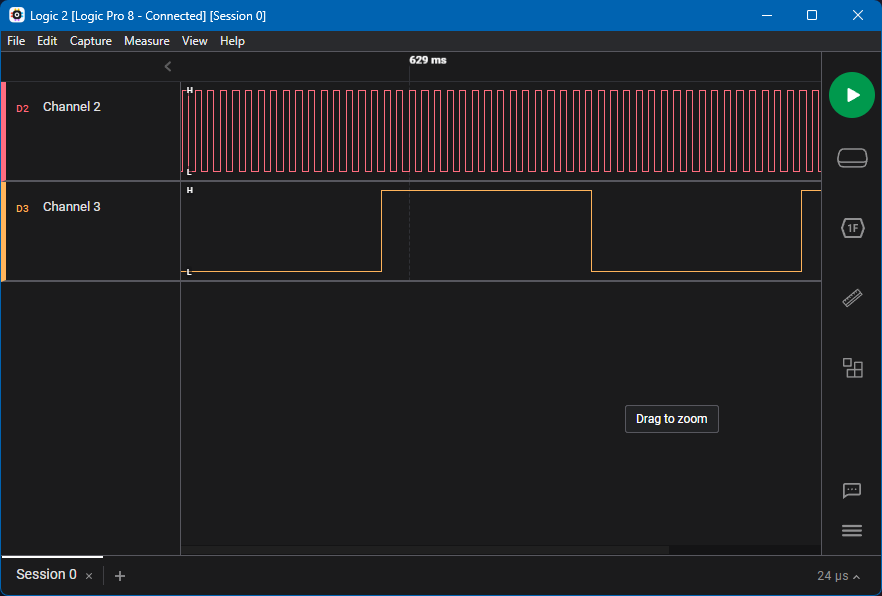
\includegraphics[width=.8\textwidth]{Figures/4_controlsystem_stm32_zephyr.png}
	\caption{STM32 Zephyr RTOS pulser output}
	\label{fig:4_stm32_zephyr_pulser}
\end{figure}
During the initial implementation stage of the control system, a bring-up of the STM32F411RE board and several pulse signals were succesfully generated. In \cref{fig:4_stm32_zephyr_pulser}, two pulse signals can be seen. In Channel 2, \qty{5}{\mega\hertz} ultrasound pulse can be seen. In Channel 3, the \qty{10}{\kilo\hertz} PRF signal can be seen. Unfortunately, soon thereafter it was discovered a limitation of the API in Zephyr is not mature enough developed for power systems such as the half-bridge in the transmitter circuit. In more practical terms, it was not possible to generate two complementary signals with dead-time using the existing Zephyr PWM API. To continue with that solution, a new PWM driver would have to be written from scratch, which is no trivial task. Alternative solutions were investigated. Another option was to use the \gls{hal} provided by the manufacturer of the microcontroller. However, it was decided to try an alternative system known as PYNQ Z1, which is a development board by Agilent. On the PYNQ Z1 board is a Zynq 7000 \gls{soc}. Inside the Zynq 7000 SoC there are both an \gls{fpga} and Arm based processor.

\section{Power Stage}
\begin{figure}[htbp]
	\centering
	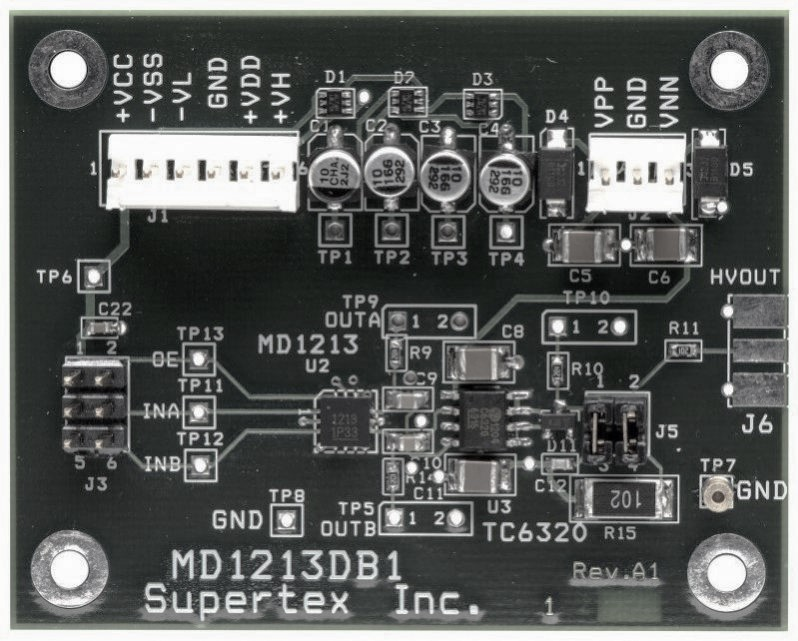
\includegraphics[width=.8\textwidth]{Figures/4_transmitter_pcb_pic.jpg}
	\caption{MD1213DB1 High Speed Pulser}
	\label{fig:4_transmitter_pcb_pic}
\end{figure}
A picture of the power stage PCB can be seen in \cref{fig:4_transmitter_pcb_pic}. An experiment is conducted to validate the function of the power stage. Using the jumpers, the PCB is configured without its onboard load, and a \gls{pzt} transducer is attached with a splitter adapter to connect the other side to an oscilloscope for data acquisition.

\section{Transmit/Receive Switch}
\begin{figure}[htbp]
	\centering
	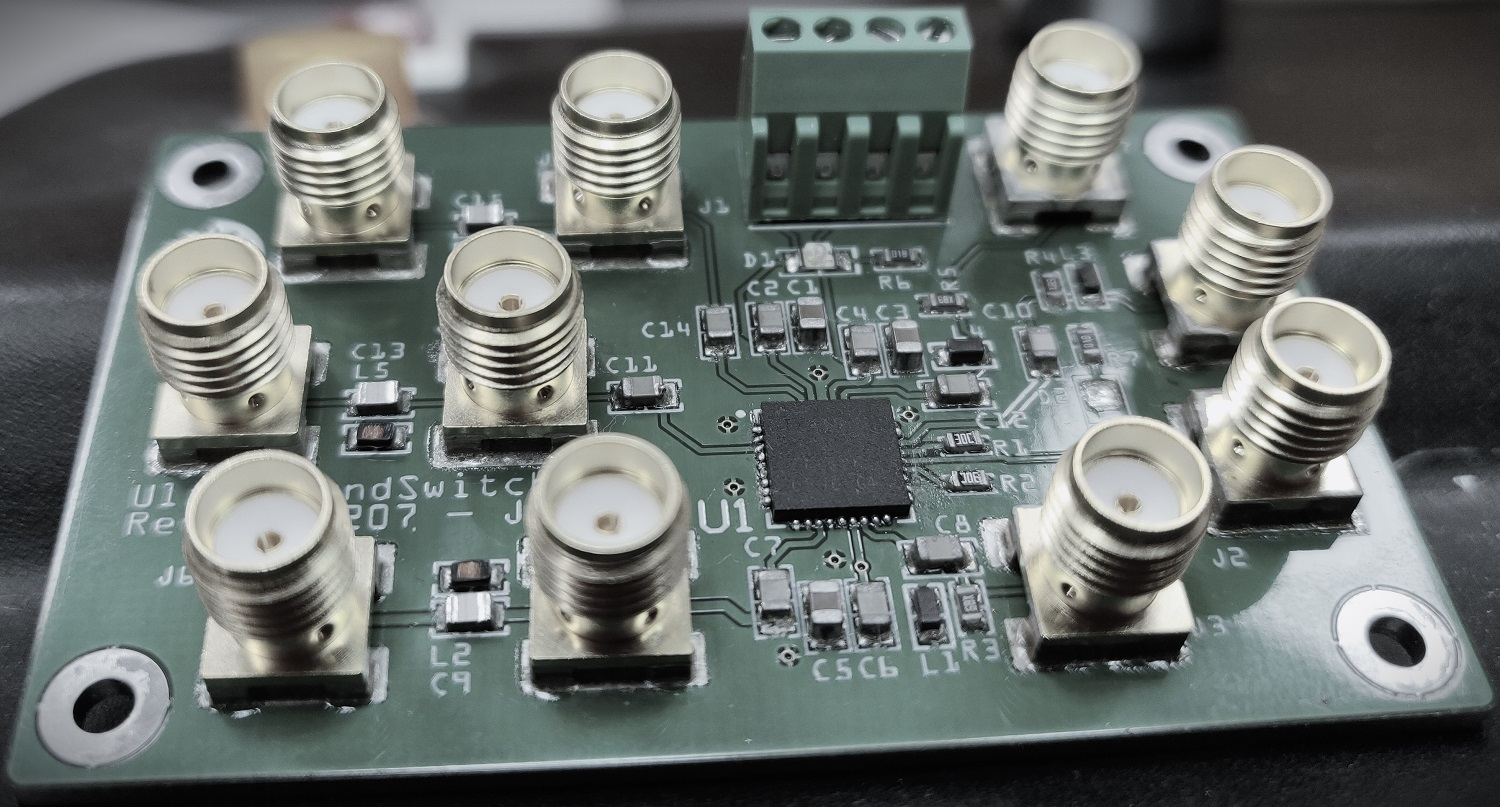
\includegraphics[width=.8\textwidth]{Figures/4_switch_pcb_pic.jpg}
	\caption[Transmit/Receive Switch after assembly]{Transmit/Receive Switch after assembly}
	\label{fig:4_txrx_pcb}
\end{figure}
The entire schematic of the transmit/receive switch can be found in the appendix in \cref{fig:appendix_ultrasoundswitch_a,fig:appendix_ultrasoundswitch_b}. As mentioned in the previous chapter, a PCB layout was made and a batch of 5 was ordered with an accompanying stencil for fast assembly. After the PCBs arrived, the stencil was mounted in the stencil frame and the PCB was aligned for solder paste application. After the solder paste application is completed, all the components are placed on their corresponding footprints and the PCB is placed in the reflow oven. The equipment used in this process is listed in \cref{tab:instruments_solder_work}. The finished assembly can be seen in \cref{fig:4_txrx_pcb}.


\section{Band-Pass Filter}
Since the \gls{bp} filter is comprised of a module component in a bespoke form factor, a circuit is implemented on a prototyping board. With the BPF-C4R5+ mounted in the center, input and output connectors are placed on either side with SMA connectors. Since the filter is passive, no power connectors are needed.

\section{Preamplifier}
Before the signal can be demodulated, it must be DC-biased and amplified. This is what the preamplifier is for. For the preamplifier, the circuit is validated using an experiment where a function generator is transmitting a low amplitude sine with ac-coupling and measure the amplified dc-coupled output.

\section{Quadrature Demodulator}
\begin{figure}[htbp]
	\centering
	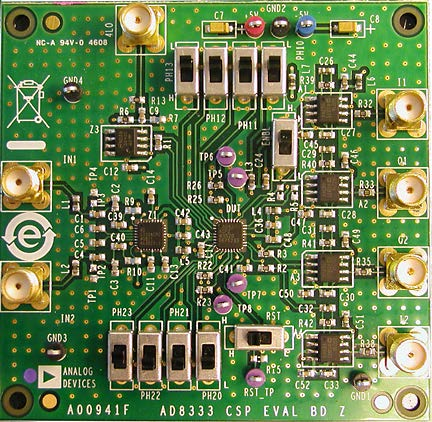
\includegraphics[width=.8\textwidth]{Figures/4_demod_pcb_pic.jpg}
	\caption{Demodulator PCB AD8333-EVALZ}
	\label{fig:4_demod_pcb_pic}
\end{figure}
As described in the previous chapter, the demodulator use an I/Q quadrature demodulation scheme to take two differential RF signals and a quadruple frequency signal, in this case, \qty{5}{\mega\hertz} and \qty{20}{\mega\hertz}, respectively, and determines the frequency difference between the fundamental frequency and the Doppler frequency on the output.
The entire schematic of the demodulator can be found in the appendix in \cref{fig:appendix_ad8333}.
\section{Sample and Hold}
After each demodulated burst is sampled, between each sample line pulse repetition it is desired to hold the voltage, so the analogue-to-digital conversion that may be running asynchronously does not sample zero-values between the bursts. Therefore, an experiment is conducted with the sample-and-hold amplifier to verify the functionality. A low-frequency I-Q simulated signal is created from the function generator with a sample gating pulse train to control the sample-and-hold function.

\section{Pulse-Repetition and Wall Filter}
\section{Digital Signal Processor}


%\begin{figure}[H]
%	\centering
%	\begin{circuitikz}[american voltages]
%		\draw
%		(0,0) to [short, *-] (6,0)
%		to [V, l_=$\mathrm{j}{\omega}_m \underline{\psi}^s_R$] (6,2)
%		to [R, l_=$R_R$] (6,4)
%		to [short, i_=$\underline{i}^s_R$] (5,4)
%		(0,0) to [open, v^>=$\underline{u}^s_s$] (0,4)
%		to [short, *- ,i=$\underline{i}^s_s$] (1,4)
%		to [R, l=$R_s$] (3,4)
%		to [L, l=$L_{\sigma}$] (5,4)
%		to [short, i_=$\underline{i}^s_M$] (5,3)
%		to [L, l_=$L_M$] (5,0);
%	\end{circuitikz}
%	\caption{The nodes short, V, R and L are presented here, but there a lot more}
%	\label{fig:circuitikz}
%\end{figure}
%
%\section{Listings (code)}
%
%\Cref{lst:helloworld} is a nicely formatted block of code. A listing will automatically continue on the next page if it encounters a page break. Many different programming languages can be highlighted. Check the \texttt{listings} package documentation for a list of supported programming languages.

%\begin{listing}[htbp]
%\begin{mintedc}
%#include <stdio.h>
%int main()
%{
%	printf("Hello, World!"); /*printf() outputs the quoted string*/
%	if (n == 0 || n == 1){
%		return n;
%	}
%	j = 0;
%	for (i = 0; i < n-1; i++){
%		if (arr[i] != arr[i+1]){
%			arr[j] = arr[i];
%			j++;
%		}
%	}
%	arr[j++] = arr[n-1];
%	return 0;
%}
%\end{mintedc}
%	\caption{Hello world in C}
%	\label{lst:helloworld}
%\end{listing}



